% !TeX root = ../main.tex
% Add the above to each chapter to make compiling the PDF easier in some editors.

\chapter{Background}\label{chapter:background}

This chapter discusses the relevant background knowledge required to understand the remainder of this work.

\section{Trusted execution environment}

One of the core security concepts of operating systems are the privilege levels of processes. Thereby, processes are protected against other processes with the same privilege level. However, they are not protected against more privileged processes. This bears problems for example for cloud computing and edge computing. In cloud computing, other services, the hypervisor, or the cloud provider in general could potentially access sensitive data of the cloud tenant. In edge computing, the edge applications deal with plain text data, while they are potentially running on insecure edge devices. Hence, protection against more privileged processes is desired.

A \ac{TEE} is an integrated hardware extension to processors. Effectively, the execution environment is separated into the \ac{REE} and the \ac{TEE}. The \ac{REE} runs the common software, e.g., a Linux-based operating system and the applications. The TEE allows code to be executed and memory separately to be used on a device in a hardware-protected manner that ensures a high level of confidentiality and integrity. Therefore, it aims to protect data-in-use, instead of data-in-transit or data-at-rest. Since it is integrated into the processor, there is no separate chip required. However, it is common to give the \ac{TEE} a dedicated volatile memory chip, namely the secure RAM~(sRAM), which is ensured to be exclusively accessible to the \ac{TEE} by hardware.

Moreover, the \ac{TEE} commonly follows the same user and kernel space separation as \ac{REE} operating systems. The kernel space is running a trusted OS kernel, and the user space is running the trusted applications.

One such \ac{TEE} is ARM's TrustZone~\cite{ARM09}. It partitions all software and hardware resources of the containing system into the Normal world~(NW) and the Secure world~(SW).
While the SW can access the resources of the SW and the NW, the NW is restricted to its own resources.
Since ARM is the dominant processor architectures for IoT devices with a market share of 86\,\% \cite{eclipse}, many of the approaches in this field of research rely on ARM technology such as TrustZone.
Our approach also leverages TrustZone to enable the execution and the remote attestation of an fTPM.

Other common \ac{TEE} technologies are Intel Software Guard Extensions (SGX), Intel Trusted Domain Extensions (TDX) and AMD Secure Encrypted Virtualization (SEV). Since we focus on the implementation of our concept with ARM TrustZone, we do not go into detail about these other technologies here. However, since our concept is not tied to ARM processors and can also be applied to others, they are mentioned for the sake of completeness.

\section{Attestation}
\subsection{Local attestation}
\subsection{Remote attestation}

Remote attestation is a challenge-response protocol initiated by a remote attestor.
The challenge contains a nonce, enforcing a fresh response.
The response must be a proof of the challenged system that it is trustworthy.

TPMs send PCR values in the form of a digitally signed quote to a remote attestor.

Remote attestation is the process initiated by a remote trusted party (called ``verifier'') to verify that an end-device (called ``prover'') has not been tampered with. For detecting that, remote attestation generally inspects the following properties of a program: (i) its code and data has been correctly loaded into memory for execution, (ii) its execution has not been redirected in unintended ways at runtime, and (iii) its data has not been maliciously modified at runtime.

A trusted anchor is required on the device to be attested because at least one trusted component is necessary to extract the data from the remote device to be verified. In many cases, TEE's act as a trust anchor because they are hardware-protected, making it an excellent candidate for a trust anchor.

\section{Trusted Platform Module}

TPMs support three main use-cases: secure key generation, remote system attestation, and secure storage. 

There are various types of TPMs. They all offer the same functionality, but with different security guarantees and are also deployed differently.

% From https://www.usenix.org/system/files/conference/usenixsecurity18/sec18-han.pdf
% Rephrase
Allows remote attestation with PCR values in the form of a digitally signed quote to a remote attestor.

% PCR usage table (similar to https://www.usenix.org/system/files/conference/usenixsecurity18/sec18-han.pdf)

$PCR(i)_{t+1} = hash(PCR(i)_t\ |\ new\ measurement),\ PCR(i)_0 = 0$

% Maybe add graphs for dTPM and vTPM:
% CPU <-LPC-> dTPM
% [CPU|TEE[fTPM]]

\begin{figure}
    \begin{subfigure}{0.49\textwidth}
      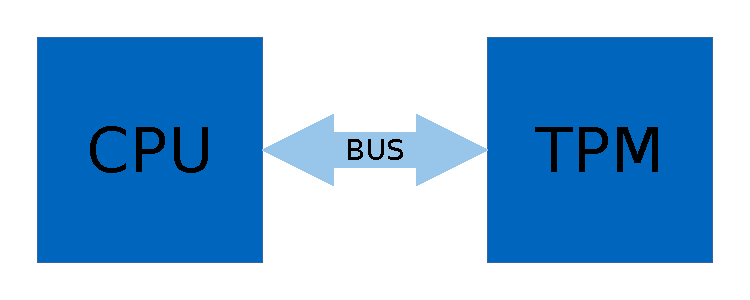
\includegraphics[width=\linewidth]{figures/dTPM.pdf}
      \caption{Discrete TPM} \label{fig:dtpm}
    \end{subfigure}%
    \hspace*{\fill}   % maximize separation between the subfigures
    \begin{subfigure}{0.49\textwidth}
      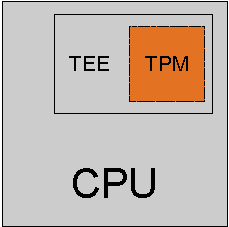
\includegraphics[width=\linewidth]{figures/fTPM.pdf}
      \caption{Firmware TPM} \label{fig:ftpm}
    \end{subfigure}%
  
  \caption{Schematic illustration of the different TPM types.} \label{fig:tpm_types}
  \end{figure}

\subsection{Discrete TPM}

This is the classical form of a TPM. It is a dedicated piece of hardware, connected to the CPU via a bus. It is designed and manufactured to be highly temper-resistant against hardware attacks.
% Reference https://www.intel.de/content/dam/www/program/design/us/en/documents/low-pin-count-interface-specification.pdf

The well known TPM Reset Attack was independently described in \cite{kauerBernhard,sparks2007}. It requires minimal hardware, precisely only a wire connecting the data signal of the LPC bus to ground. This results in a reset signal for the TPM, yielding predictable values for the PCR registers, i.e., 0. This allows an attacker to replay arbitrary register extends.

Winter and Dietrich \cite{Winter2013} show attacks against the bus between a TPM and the CPU. They built-up onto the previously described TPM Reset Attack. It focuses on resetting the PCR values by active hardware attacks, while the running platform does not change. For that, a valid boot procedure is required to retrieve the valid PCR values. However, it also introduces the opposite, where the PC is reset, and an evil operating system/firmware booted, but the TPM is not aware of this, keeping the valid PCR values of the previous boot procedure.

\cite{Kursawe2005AnalyzingTP} also attacks LPC bus against TPM 1.1. They observed that the data of some operations like unsealing are transmitted via the bus in plain text.

Invasive hardware attacks on dTPMs have already been shown in 2010 by Tarnovsky \cite{tarnovsky}. However, this requires a lot of time, knowledge, and resources, i.e., hardware and money.

Also, I2C common for bus system. Hardware interface even standardized by TCG.

% LPC most common for PC clients
% I2C most common for embedded clients (SPI too?)
% LPC, I2C and SPI defined in https://trustedcomputinggroup.org/resource/pc-client-platform-tpm-profile-ptp-specification/

\subsection{Firmware TPM}

As seen in the previous section, the bus between the CPU and a TPM is the biggest attack vector. An fTPM circumvents this by being directly executed within the CPU, revealing no easily accessible bus.

\subsection{Virtual TPM}



\section{Secure Boot and Measured Boot}

Secure boot is a concept of UEFI doing local attestation of components directly at boot-time. Based on signatures of next-to-boot components. It cancels the boot process as soon as deviations are detected. Binaries of components are first signed and then, deployed universally. Hence, binaries are not bound to the platform and can be considered portable in this context.

Measured Boot is a concept that is often implemented in interplay with a TPM. Measured Boot allows remote attestation to a later time. Uses sealing functionality of TPMs, therefore, bound to the exact platform.

Both technologies are often used in conjunction.
